\clearpage
\section{Help Desk Implementation}\label{implementation}
The main class of artifacts produced by this project is the cloud help desk system. Furthermore, artifacts are either non-technical (thus requiring no specific competencies to understand) or technical. Finally, all results must be \textit{\gls{smart}}.

\subsection{Technical Artifacts}\label{technical}
Several technical artifacts must be created to satisfied fulfill the \textit{\gls{perc}} request. The activities, within Giglium are responsible to make in time are described in the following subsection.

\begin{figure}[ht!]
	\centering
	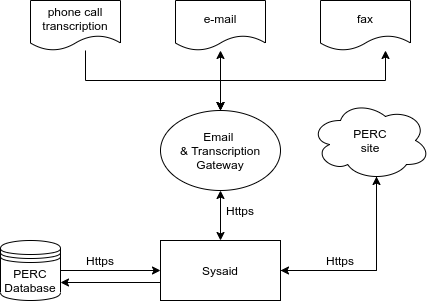
\includegraphics[width=120mm]{./img/implementations/infrastructure.png}
	\caption{High level help desk infrastructure}\label{fig:high-level-help-desk-infrastructure}
\end{figure}

\subsubsection{Sysaid Setup}\label{setup}
Giglium firmly believes in the \textit{\gls{iac}} principles, for this reason Giglium will provide a Terraform\cite{terraform} script that will create and provision two\footnote{The number of the \gls{vm} can be increased and decreased using the Terraform script to respond to high or low demand.
Giglium suggests having always two \textit{\gls{vm}}s to have a good \textit{\gls{ha}}.} \textit{Windows Server 2019} \textit{\gls{vm}}s on the Azure\cite{azure} cloud.\footnote{Azure credentials will be provided from \gls{perc}.} 
The newly created machines need to have at least 4 vCore, 8 GB RAM and 32 GB of storage\cite{sysaid_requirements} but Giglium suggests using at least the \textit{Standard-A4m-v2} tier from the Azure catalog. The Terraform script will also take care of the creation of the security group using the \textit{\gls{polp}} approach.
The Terraform script will also generate the SSH key required to enter inside the \textit{\gls{vm}}s, and it will be the only one authorized to change the state of the infrastructure. The state and all the sensitive data will be store inside the autogenerated \texttt{.tfstate} file.\gls{perc} will be responsible to store this file safely. 

Once the \gls{vm}s will be up and running, the Terraform script will call an Ansible\cite{ansible} script to finish the provisioning. This script will configure the SysAid cluster, and it will safely expose its \textit{\gls{api}}. The ansible script will also connect, using SSH, to the machine provided by \textit{\gls{perc}} to install the database. Giglium will install SQL Server 2019, for this reason, the provided machine needs to follow these requirements\cite{sql_requirements}\footnote{Giglium strongly recommended to have at least 4 GB RAM.}. All the backups for this database will be the responsibility of \gls{perc}.

\begin{figure}[ht!]
	\centering
	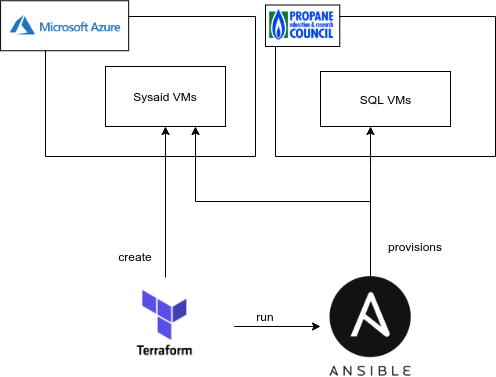
\includegraphics[width=120mm]{./img/implementations/setup.png}
	\caption{High level infrastructure set up}\label{fig:high-level-infrastructure-set-up}
\end{figure}

\paragraph{SysAid Orchestrations} To helps to automate manual, error-prone, routine tasks, Giglium will create some rules and automated actions to slash the ticket resolution time. All these configurations will be used to configure Automate Joe the native orchestrator of SysAid. Giglium will perform an initial analysis to understand the best actions to put in place. 

\paragraph{SysAid custom \textit{\gls{api}}} To connect Sysaid \textit{\gls{kb}} with the \textit{\gls{st}} Online Resource\cite{propanesafety}, Giglium will expose the Sysaid \textit{\gls{api}}. To be able to query the \textit{\gls{api}}, first of all \gls{perc} will need to login, following the procedure described here:\cite{sysaid_api_login}. Once retrieved the \texttt{JSESSIONID} token, \textit{\gls{perc}} will be able to query the following custom endpoint:

\begin{table}[h!]
	\begin{center}
		\begin{tabularx}{\linewidth}{l|X|X|}
			\toprule
			\textbf{Command Name} & \textbf{Command} & \textbf{Description}\\
			\midrule 
			Get Articles List & GET/articles?fields={field1,field2..} 
			\&offset={offset}\&limit={liqueuesmit} &  Return all articles inside the \textit{\gls{kb}}\\[10ex]
			Get Article       & GET/articles/{id}?fields={field1,field2..} & Return a specific article inside the \gls{kb}\\
			
			\bottomrule
		\end{tabularx}
		\caption{Custom \gls{api} table}\label{tab:api}
	\end{center}
\end{table}

\subsubsection{Setting up faxing in Exchange Online}\label{fax_setup}
Giglium will configure Microsoft 365 Exchange Online to receive the fax data and then sends it to SysAid with the fax included as a \texttt{.tif} attachment. Microsoft 365 Exchange Online will be also configured to receive an email composed with the main body of the email with the fax information and with attached a \texttt{.pdf} file that will be converted into the fax.

\subsubsection{Libraesva Setup}\label{libraesva_setup}
Libraesva will be our active defense against cybercrime. Giglium will configure Microsoft 365 with Libraesva as our inbound and outbound mail gateway. To be sure all the email, fax, and calls transcription will be filtered. 

\begin{figure}[ht!]
	\centering
	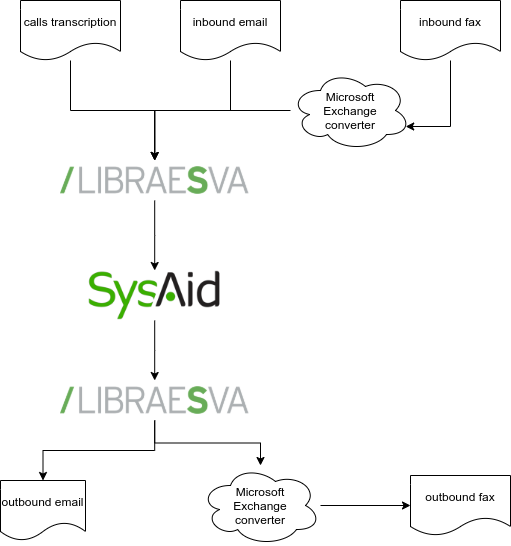
\includegraphics[width=120mm]{./img/implementations/io.png}
	\caption{Sysaid Inbound and Outbound flow}\label{fig:sysaid-flow}
\end{figure}

\subsubsection{Windows Autopilot Setup}\label{autopilot_setup}
Giglium will configure Windows autopilot to set up and pre-configure new devices or reset, repurpose, and recover devices. Windows Autopilot will:

\begin{itemize}
	\item automatically join devices to \textit{\gls{ad}};
	\item restrict the Administrator account creation;
	\item install all the necessary softwares;
\end{itemize}

\subsubsection{Microsoft 365 Teams Voice Setup}\label{365_setup}
Giglium will configure Microsoft 365 Teams Voice with a call queue that provides:

\begin{itemize}
	\item a greeting message;
	\item music while people are waiting on hold in a queue;
	\item a \textit{\gls{fifo}} call routing;
	\item some options to manage for queue overflow and timeout.
\end{itemize}

\subsection{Non-Technical Artifacts}\label{not_tecnical}
A non-technical artifacts must be configured to satisfied fulfill \textit{\gls{perc}} request. The activities, within Giglium are responsible to make in time are described in the following subsection.

\subsubsection{Help Desk User Workspace Kit}
To ensure a more flexible and cost-saving help desk, Giglium has built a strong cloud-based infrastructure. This will permit all help desk users to work from home. The minimum requirements are an internet connection and a laptop. Work from home has several benefits for business, such as:
\begin{itemize}
	\item Increased staff motivation {-} by working from home staff will feel more trusted by their employer as the working relationship isn't as closely monitored and employees are allowed a degree of autonomy to get on with their work.
	\item Financial benefits {-} savings on office space, office supplies, utility bills, and other facilities.
	\item Fewer sickness absences {–} staff are more likely to feel happier and more energized working from home and therefore less chance of their immune system is negatively impacted by burnout. Also, the fact that employees are working in isolation there is less chance of infections spreading as would be the case within an office environment.
\end{itemize}

Giglium will be responsible to put in place a workspace kit with adequate hardware. 
Every help desk operator will have the Dell laptop: \textquotedblleft New Inspiron 15 3000\cite{dellpc}\textquotedblright with 3 Years Hardware Warranty with Onsite/In-Home Service after Remote Diagnosis. The laptop specification with a CPU AMD Ryzen™ 5\cite{amdcpu} and 8 GB RAM overlap the Microsoft 365 Business Voice requirements but Giglium strongly recommended it to reduce the normal loss of performance over time.  
In combination with their laptop, the help desk user will have the Jabra headset: \textquotedblleft EVOLVE 2 40\cite{jabraheadsets}\textquotedblright. Thanks to their outstanding noise isolation and the Microsoft Team optimization and certifications they are perfect to provide high-quality calls with students. 
Inside the kit, every operator will find a \textquotedblleft work from home\textquotedblright guideline that will help them to create the perfect workspace.


\subsection{Timeline}
Giglium is proposing an aggressive yet feasible schedule for completing the Help Desk project.
The key milestones and deliverables are summarized below. All
deliverables will have a two-week approval period during which the Giglium project
team will address any deficiencies or concerns. Following the approval, \textit{\gls{perc}} will be invoiced for each new requisites.
\bigskip


\begin{table}[H]
	\begin{ganttchart}[vgrid={draw=none, dotted}]{1}{18}
		\gantttitlelist{1,2,3}{6} \\
		\ganttgroup{Technical Artifacts}{1}{18} \\
		\ganttbar[name=svms]{Sysaid \gls{vm} Setup}{1}{12} \\
		\ganttbar[name=soc]{Sysaid Orchestrations Setup}{14}{18} \\
		\ganttbar[name=sapi]{Sysaid \gls{api} Setup}{14}{18} \\
		\ganttlink{svms}{soc}
		\ganttlink{svms}{sapi}
		
		\ganttbar[name=was]{Windows Autopilot Setup}{1}{12} \\
		\ganttbar[name=mtvs]{Microsoft 365 Teams Voice Setup}{14}{18} \\
		\ganttbar[name=ls]{Libraesva Setup}{14}{18} \\
		\ganttbar[name=feo]{Setting up faxing in Exchange Online}{14}{18} \\
		\ganttlink{was}{mtvs}
		\ganttlink{was}{ls}
		\ganttlink{was}{feo}
		
		\ganttgroup{Non-Technical Artifacts}{1}{18} \\
		\ganttbar{Help Desk User Workspace Kit}{1}{18} \\
	\end{ganttchart}
	\caption{Macro-plane chart}\label{tab:gantt}
\end{table}

In the chart~\ref{tab:gantt} we can find the macro-plane, divided into weeks. As we can see three weeks are necessary to have the whole help desk project configured. The macro plan will be more detailed and possibly modified by the Project Manager after the sign of the proposal.

\subsection{Service Delivery}
For the delivery of the help desk product described in this section, the delivery of the
service will take place according to the \textit{\gls{raci}} table~\ref{tab:i_sd_raci}.

\paragraph{Table legend:}
\begin{itemize}
	\item Responsible (\textbf{R}): executor of the activity;
	\item Accountable (\textbf{A}): responsible for the result of the activity;
	\item Consulted (\textbf{C}): provides input
	\item Informed (\textbf{I}): informed on the execution of the activity.
\end{itemize}

\begin{table}[H]
	\centering
	\begin{tabular}{|l|l|l|l|} 
		\hline
		\textbf{Activity} & \textbf{Type} & \textbf{Giglium} & \textbf{\gls{perc}}   \\
		\hline
		Architecture Definition & Architecture & A-R  &  C  \\
		\hline
		Architecture Provisionin & Infrastructure & A-R & I  \\
		\hline
		SQL Server \textit{\gls{vm}} creation & Infrastructure & C & A-R  \\
		\hline
		Azure \textit{\gls{vm}} creation & Infrastructure & A-R & C  \\
		\hline
		Azure \textit{\gls{vm}} scale up or down & Infrastructure & A-R & C  \\
		\hline
		\textit{\gls{vm}} Provisioning script & Software & A-R & I \\
		\hline 
		Firewall setup & Software & A-R & C \\
		\hline 
		Microsoft 365 Teams Voice and Fax setup & Software & A-R & I \\
		\hline 
		Sysaid setup & Software & A-R & I \\
		\hline 
		Windows Autopilot Setup & Software & A-R & I \\
		\hline 
		Libraesva Setup & Software & A-R & I \\
		\hline 
		Minor Software patch & Software & A-R & C \\
		\hline 
		Minor Windows update & Software & A-R & C \\
		\hline 
		Integration with \textit{\gls{st}} Online Resource & Software & C & A-R \\
		\hline
		SQL Server Database Backup & System & C & A-R \\
		\hline 
		Terraform \texttt{.tfstate} file safety & System & C & A-R \\
		\hline 
		Disaster Recovery Plan & System & C & A-R \\
		\hline 
		System Monitoring for SQL Server \textit{\gls{vm}} & System & C & A-R \\
		\hline 
		System Monitoring for Azure \textit{\gls{vm}} & System & A-R & I \\
		\hline 
		Help Desk User Workspace Kit & Hardware & A-R & I \\
		\hline
	\end{tabular}
	\caption{Implementations service delivery \textit{\gls{raci}}}\label{tab:i_sd_raci}
\end{table}